\documentclass[11pt,a4paper]{article}
\usepackage{amsmath,amssymb,graphicx,geometry,hyperref,fontspec}
\geometry{margin=2.2cm}
\setlength{\parindent}{0pt}\setlength{\parskip}{4pt}
\title{Bell Programmer Manual\\\large modules, examples, structure file}
\date{\today}
\begin{document}
\maketitle
\tableofcontents
\clearpage
\section{Programmer Manual}

Physics is in the Beam Physics Manual. Architecture of the
blocks is in Architecture. This page lists entry
points of the Julia package \texttt{Bell}.

The object of the ring is the Lie product of Dragt–Finn factors.
Concatenate in the algebra, read the product, track a point through it.
Linear optics is the closed form of $\exp(:f_2:)$, stored as the matrix
$R$. It is not a second theory of the lattice.

\begin{figure}[htbp]\centering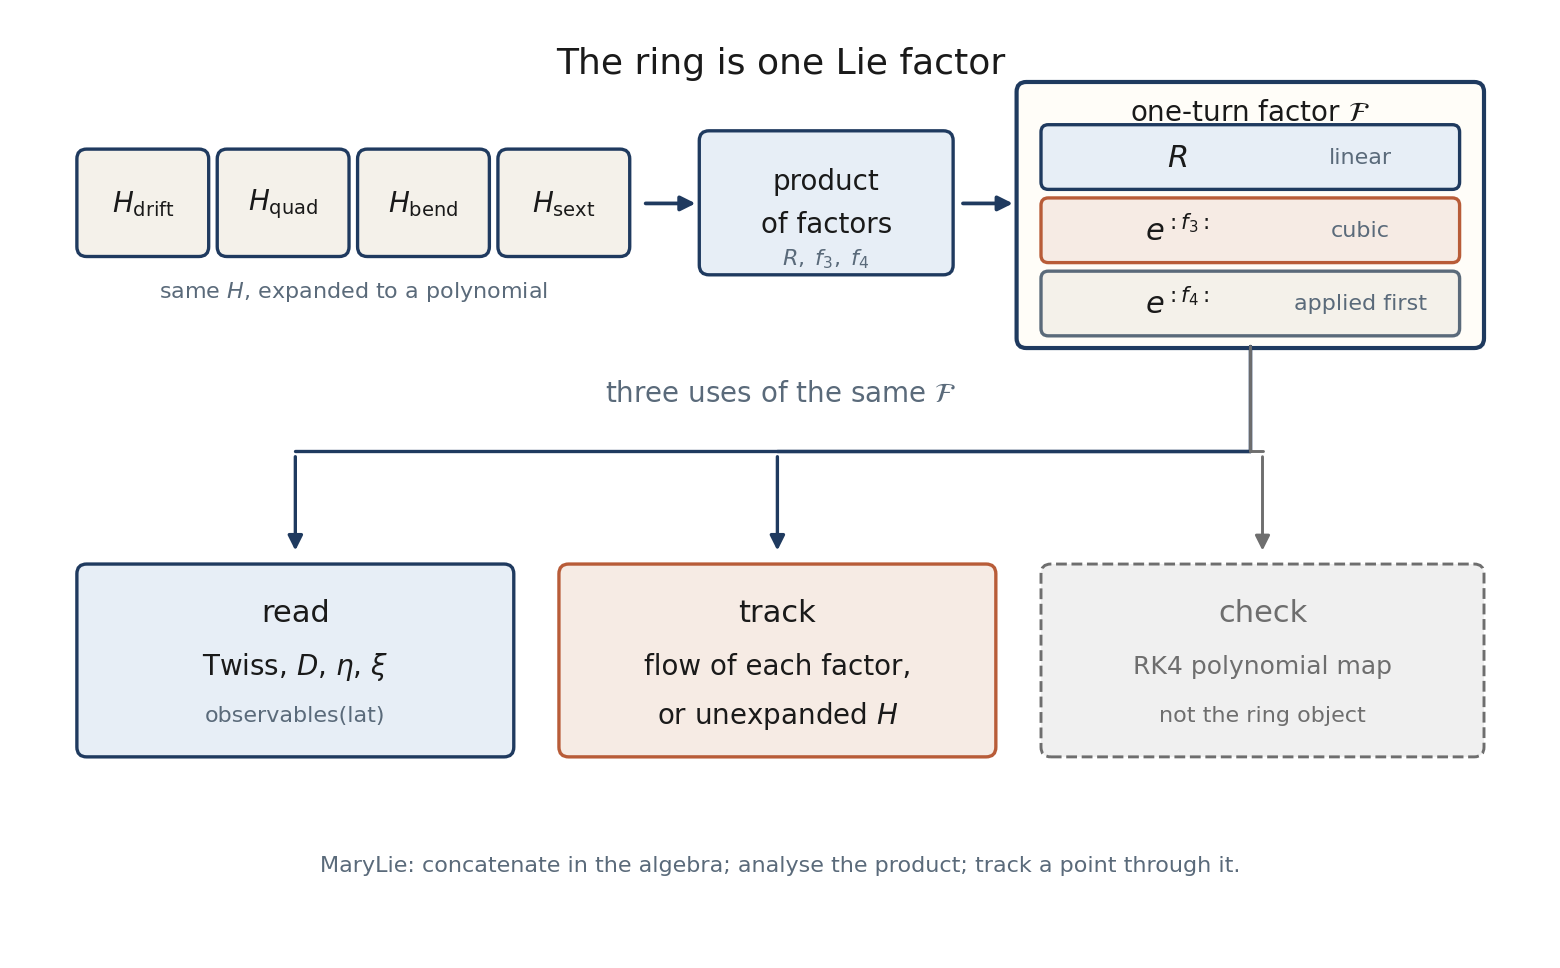
\includegraphics[width=\linewidth]{../src/assets/architecture_object.png}\caption{The ring is one Lie factor: Hamiltonians are concatenated in the algebra; the product is read, tracked, or checked.}\end{figure}

\texttt{observables(lat)} builds \texttt{ring\_lie\_factor} once and reads Twiss,
$\eta$ and $\xi$ from that factor. \texttt{ring\_taylor\_map} is an RK4
polynomial and is not that object.

\begin{figure}[htbp]\centering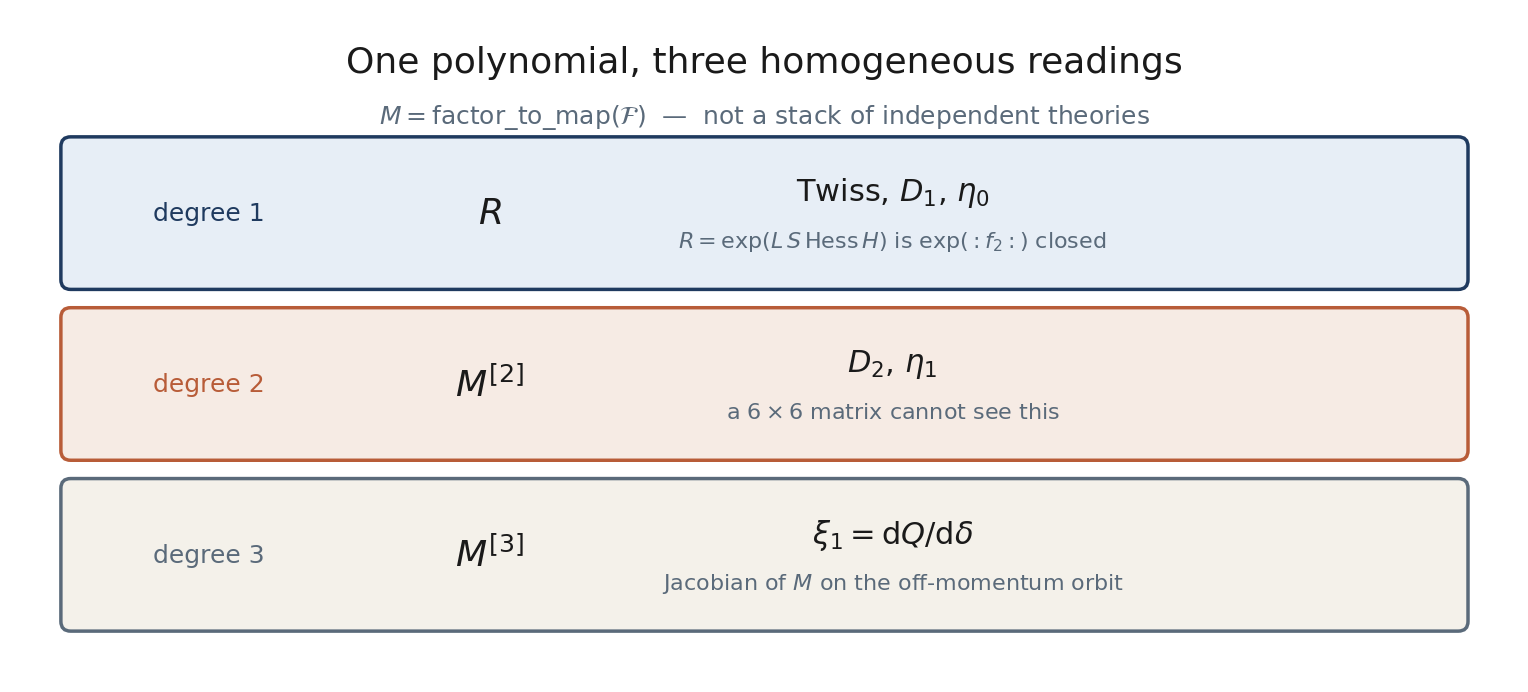
\includegraphics[width=\linewidth]{../src/assets/architecture_orders.png}\caption{One polynomial, three homogeneous readings: degree 1 gives Twiss and $\eta_0$; degree 2 gives $D_2$ and $\eta_1$; degree 3 gives $\xi_1$.}\end{figure}

\subsection{Layout}

\begin{center}\small\begin{tabular}{p{0.475\linewidth}p{0.475\linewidth}}\hline
\textbf{path} & \textbf{role}\\\hline
\texttt{src/coordinates.jl} & particle, reference, $v(\delta)$, $e(\delta)$, $z\leftrightarrow u$\\
\texttt{src/elements.jl} & element types (data only)\\
\texttt{src/structure.jl} & structure file, \texttt{Lattice}, sequence edits\\
\texttt{src/hamiltonians.jl} & element generator $H$ as a polynomial\\
\texttt{src/lie\_algebra.jl} & polynomial space, Poisson bracket, Dragt–Finn product\\
\texttt{src/optim\_converter.jl} & writes a structure file from OptiM $.opt$\\
\texttt{src/linear.jl} & $R=\exp(L S \mathrm{Hess}\,H)$, slice Twiss along $s$\\
\texttt{src/symplectic.jl} & $J^\mathsf{T}SJ-S$\\
\texttt{src/tracking.jl} & flow of each factor, thin RF kick, product of the ring\\
\texttt{src/higher\_order.jl} & closed orbit, $D_2$, $\eta$, chromaticity, \texttt{observables}\\
\texttt{src/differential\_algebra.jl} & independent DA map (RK4 in polynomials) — a check\\
\texttt{src/normal\_form.jl} & one-turn factor with thin RF; torus average of $\delta$\\
\texttt{src/longitudinal.jl} & averaged longitudinal Hamiltonian in $(\varphi,\delta)$\\
\texttt{src/exact\_integrator.jl} & unexpanded $H$, finite cavity, renormalise\\
\texttt{src/acceleration.jl} & ramp, tune fit\\
\texttt{src/plotting.jl} & figures\\
\texttt{src/optimizers.jl} & optional sextupole response\\
\texttt{src/Bell.jl} & loads every block and re-exports\\
\hline\end{tabular}\end{center}

Entry: from the \texttt{Julia} folder, \texttt{using Bell}.

The one-turn object used for the normal form is \texttt{one\_turn\_factor\_rf}.
Optics of the magnetic product without RF is \texttt{observables(lat)}.

\subsection{Examples}

\begin{verbatim}
julia --project=. examples/10_linear_optics.jl
julia --project=. examples/11_lie_maps.jl
julia --project=. examples/12_higher_order.jl
julia --project=. examples/13_optional_sextupole_optimization.jl
julia --project=. examples/14_rf_acceleration.jl
julia --project=. examples/15_coordinates.jl
julia --project=. examples/16_blond_longitudinal.jl
julia --project=. examples/17_lie_product.jl
julia --project=. examples/18_lie_normal_form.jl
\end{verbatim}

The equilibrium-momentum study lives in \texttt{C:\textbackslash{}GIT\_REPOS\textbackslash{}SCT\_2\textbackslash{}Julia\textbackslash{}equilibrium\_energy}.
It depends on this package via \texttt{Pkg.develop} of the \texttt{Julia} folder.

\subsection{Accepted design choices}

- Injection kinetic energy 10 MeV; final 270 MeV from the lattice header.
- Stationary study: thin RF, $V=0.2$ MV, $h=5$, $\varphi_s=\pi$.
- Ramp demo: finite cavity $L=1$ m, $\varphi_s=150^\circ$.
- Mass = CODATA deuteron $1875.61294257$ MeV (OptiM \texttt{Mass=2*938.272} ignored).
- Lattice sequence used once (file \texttt{Number of periods=2} is an error; bend is 360 deg).
- Closed $D(0)=0.011$ m (OptiM initial 0 is not the closed solution).
- Default sextupole strengths are zero.

\subsection{Docs build}

\begin{verbatim}
julia --project=docs docs/make.jl
\end{verbatim}

Developer: Kolokolchikov Sergey Dmitrievich, sergey.bell13@gmail.com.

\end{document}
